%%%%%%%%%%%%%%%%%%%%%%%%%%%%%%%%%%%%%%%%%%%%%%%%%%%%%%%%%%%%%%
%% 卒論サンプル 2015.10.26, 2016.11.2, 2017.11.1, 
%% 2018.10.31, 2021.10.27, 2022.11.4 改 I. KIKUMASA
%%・ラベルを使っているので TeX に2回かけること!
%% (T2P または T2R ボタン)
%%・titlepage_a4j.tex ファイルを同じフォルダに置いておくこと!
%%%%%%%%%%%%%%%%%%%%%%%%%%%%%%%%%%%%%%%%%%%%%%%%%%%%%%%%%%%%%%
\documentclass[a4j,12pt]{jarticle}
\usepackage{amsmath}					% AmS-LaTeX を使うなら
\usepackage{amsthm}						% 定理環境のため
\usepackage{bm}								% もしエラーになるならこの行は削除してもよい。
\usepackage{amssymb}					% AmS-LaTeX を使うなら
%\usepackage{type1cm}					% タイトルに数式を使うならここを有効にして!

\usepackage{amsfonts}
\usepackage[bbgreekl]{mathbbol}
% 数字の mathbb

\usepackage[dvipdfmx]{graphicx}
\usepackage{tikz}
\usetikzlibrary{positioning, intersections, calc, arrows.meta,math}

%% 定理環境の定義
% テキストp.46「§2.4.2 定理環境の定義」参照
\theoremstyle{definition}
\newtheorem{theorem}{定理}[section]
%\newtheorem{theorem}{定理}		% セクション番号を付けないならこちら
\newtheorem*{theorem*}{定理}	% * 付きは定理番号が付かない
\newtheorem{lemma}[theorem]{補題}
\newtheorem{corollary}[theorem]{系}
\newtheorem{definition}[theorem]{定義}
\newtheorem{example}[theorem]{例}
\newtheorem{problem}[theorem]{問}
\newtheorem{axiom}[theorem]{公理}

\newcommand{\yslant}{0.4}
\newcommand{\xslant}{-0.6}

% 必要なら他にも補題や命題, * 付き等を定義せよ。

%% 証明環境
\makeatletter
\renewenvironment{proof}[1][(証明)]{\par
% 必要ならば[(証明)]を[\textbf{証明.}]等と変更することもできる。
  \normalfont
  \topsep6\p@\@plus6\p@ \trivlist
  \item[\hskip\labelsep{#1}]\ignorespaces
}{\hfill$\square$\endtrivlist}	% 証明終了の記号□を最後に付ける
%}{\endtrivlist}								% □を付けないようにしたければこちら
\makeatother

% 数式の番号をセクション番号なしにしたければ, 次の式をコメントアウト(削除)する。
% (amsmath を仮定している)
\numberwithin{equation}{section}

%% 関数記号の定義例(amsmath を仮定している)
%% 添え字を使う命令には * を付ける:
\DeclareMathOperator*{\ob}{ob}
\DeclareMathOperator*{\mor}{mor}
\DeclareMathOperator*{\dom}{dom}
\DeclareMathOperator*{\cod}{cod}
\DeclareMathOperator*{\U}{U}

%% 数式中の太字とブラックボードボールド体の定義
% 数式中の太字は $ \bm{v} $ などとすればよい。
% 複素数体は $ \CC $, 整数全体は $ \ZZ $ とかける。
\providecommand{\bm}[1]{\boldsymbol{#1}}
\providecommand{\bmdefine}[2]{\newcommand{#1}{\bm{#2}}}
\newcommand{\CC}{\mathbb{C}}
\newcommand{\RR}{\mathbb{R}}
\newcommand{\QQ}{\mathbb{Q}}
\newcommand{\ZZ}{\mathbb{Z}}
\newcommand{\NN}{\mathbb{N}}
\renewcommand{\AA}{\mathbb{A}}
\newcommand{\BB}{\mathbb{B}}
\newcommand{\DD}{\mathbb{D}}
\newcommand{\EE}{\mathbb{E}}
\newcommand{\MM}{\mathbb{M}}
\newcommand{\GG}{\mathbb{G}}
\newcommand{\Set}{\mathbb{Set}}
\newcommand{\Cat}{\mathbb{Cat}}
\renewcommand{\Vec}{\mathbb{Vec}}
\newcommand{\Ring}{\mathbb{Ring}}
\newcommand{\Grp}{\mathbb{Grp}}
\newcommand{\Top}{\mathbb{Top}}
\newcommand{\Mon}{\mathbb{Mon}}
\newcommand{\Tos}{\mathbb{Tos}}
\newcommand{\1}{\mathbb{1}}
\newcommand{\2}{\mathbb{2}}
\renewcommand{\.}{\hspace{2mm}}
\newcommand{\id}[1]{id_{#1}}

% よく使う太字はプリアンブル(この近所)に
% \bmdefine{\bv}{v}
% 等と定義しておいて, 本文中は $ \bv $ 等とすることもできる。

\title{圏論周圏論}
\author{つばきちゃん}

\begin{document}
\maketitle
%\coffeestainA{0.9}{0.85}{-25}{5cm}{1.3cm}
\newpage
%\coffeestainB{0.9}{0.85}{-25}{5cm}{1.3cm}

\tableofcontents
\clearpage

集合をスカラーという.

函手$(F:\mathbb{C}\rightarrow\mathbb{Set})$をベクトルと呼び,$F_\mathbb{C}$と表す.

函手$(G:\mathbb{D^{op}}\rightarrow\mathbb{Set})$をコベクトルと呼び,$G^\mathbb{D}$と表す.

双函手$(H:\mathbb{D^{op}\times\mathbb{C}}\rightarrow\mathbb{Set})$を行列と呼び,$H^\mathbb{D}_\mathbb{C}$と表す.

$F_\mathbb{C}$に$c\in \mathbb{C}$を代入したものは集合となり,$F_{(c)}$と表す.

$G^\mathbb{D}$に$d\in \mathbb{D}$を代入したものは集合となり,$G^{(d)}$と表す.

$H_\mathbb{C}^\mathbb{D}$に$c\in \mathbb{C}$を代入したものはコベクトルとなり,$H_{(c)}^\mathbb{D}$と表す.

$H_\mathbb{C}^\mathbb{D}$に$d\in \mathbb{D}$を代入したものはベクトルとなり,$H_\mathbb{C}^{(d)}$と表す.

ある集合$S$を$\hat{S}:\mathbb{1}\rightarrow\mathbb{Set}$として考え,$\hat{S}(*)=S$とすると$\hat{S}=\hat{S}_\mathbb{1}=\hat{S}^\mathbb{1}$であり,$S=\hat{S}_{(*)}=\hat{S}^{(*)}$と表すことができる,

行列$P_\mathbb{X}^\mathbb{X}$のエンドを$\displaystyle{\int P_{(x)}^{(x)}}^{dx}$と表す.

行列$P_\mathbb{X}^\mathbb{X}$のコエンドを$\displaystyle\int P_{(x)}^{(x)} dx$と表す.

米田埋め込み$\text{Hom}(A,B)$を$\Delta^{(A)}_{(B)}$と表す.

添え字がついた文字をテンソルという.つまりスカラー,ベクトルやコベクトル,行列はテンソルである.

それぞれ上付きと下付きの同じ添え字を持つテンソルは合成することができる.

\begin{example}
  行列$F^\BB_\AA$と$G^\CC_\BB$の合成はエンドを用いて次のように計算される.
  \[
    F^\BB_\AA G^\CC_\BB = \int {F^{(b)}_\AA G^\CC_{(b)}}^{db}
  \]
\end{example}
\begin{theorem}
  行列$E_\AA^\BB$と$F_\BB^\CC$,$G_\CC^\DD$にの合成には結合率が成り立つ.
  つまり,
  \begin{align*}
    E_\AA^\BB (F_\BB^\CC G_\CC^\DD) &= E_\AA^\BB \left(\int {F_\BB^{(c)} G_{(c)}^\DD}^{dc}\right) \\
    &= \int E_\AA^{(b)} \left(\int {F_{(b)}^{(c)} G_{(c)}^\DD}^{dc}\right)^{db} \\
    &= \int {\left(\int {E_\AA^{(b)} F_{(b)}^{(c)}}^{db} \right) G_{(c)}^\DD}^{dc} \\
    &= \left(\int {E_\AA^{(b)} F_{(b)}^{(c)}}^{db} \right) G_{(c)}^\DD \\
    &= (E_\AA^\BB F_\BB^\CC) G_\CC^\DD
  \end{align*}
\end{theorem}
\begin{proof}
  略記として$E_a^{(b)}F_{(c)}^{(d)}G_{(e)}^f=T_{a(c)(e)}^{(b)(d)f}$を用いる.
  
  $E_\AA^\BB (F_\BB^\CC G_\CC^\DD)=(E_\AA^\BB F_\BB^\CC) G_\CC^\DD$を示すために
  $\displaystyle\int E_\AA^{(b)} \left(\int {F_{(b)}^{(c)} G_{(c)}^\DD}^{dc}\right)^{db} = \int {\left(\int {E_\AA^{(b)} F_{(b)}^{(c)}}^{db} \right) G_{(c)}^\DD}^{dc}$
  を示す.
  
  任意の対象$x,y\in\CC$,$p,q\in\BB$に対して次の図式が可換になる.
  \begin{center}
    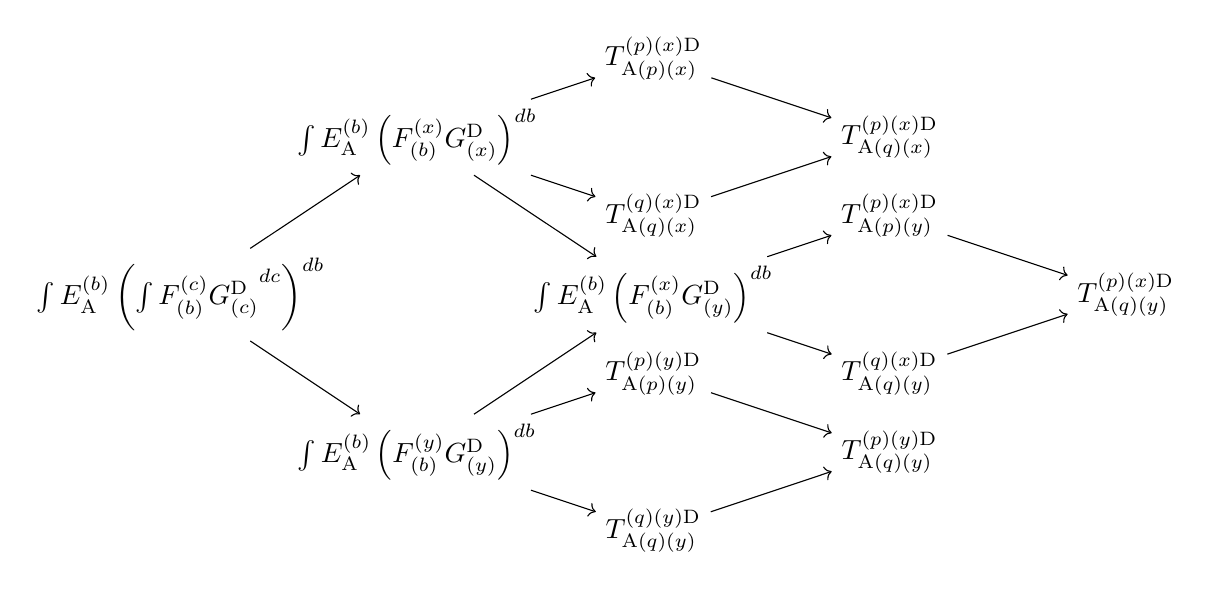
\begin{tikzpicture}
      \node (EFG1) at (0,4) {$\int E_\AA^{(b)} \left(\int {F_{(b)}^{(c)} G_{(c)}^\DD}^{dc}\right)^{db}$};

      \node (EFG2) at (3,6) {$\int E_\AA^{(b)} \left(F_{(b)}^{(x)} G_{(x)}^\DD\right)^{db}$};
      \node (EFG3) at (3,2) {$\int E_\AA^{(b)} \left(F_{(b)}^{(y)} G_{(y)}^\DD\right)^{db}$};

      \node (EFG4) at (6,4) {$\int E_\AA^{(b)} \left(F_{(b)}^{(x)} G_{(y)}^\DD\right)^{db}$};
      \node (EFG5) at (6,1) {$T_{\AA(q)(y)}^{(q)(y)\DD}$};
      \node (EFG6) at (6,3) {$T_{\AA(p)(y)}^{(p)(y)\DD}$};
      \node (EFG7) at (6,5) {$T_{\AA(q)(x)}^{(q)(x)\DD}$};
      \node (EFG8) at (6,7) {$T_{\AA(p)(x)}^{(p)(x)\DD}$};

      \node (EFG9) at (9,2) {$T_{\AA(q)(y)}^{(p)(y)\DD}$};
      \node (EFG10) at (9,6) {$T_{\AA(q)(x)}^{(p)(x)\DD}$};
      \node (EFG11) at (9,3) {$T_{\AA(q)(y)}^{(q)(x)\DD}$};
      \node (EFG12) at (9,5) {$T_{\AA(p)(y)}^{(p)(x)\DD}$};

      \node (EFG13) at (12,4) {$T_{\AA(q)(y)}^{(p)(x)\DD}$};

      \draw[->] (node cs:name=EFG1) -- node[auto=left] {} (node cs:name=EFG2);
      \draw[->] (node cs:name=EFG1) -- node[auto=left] {} (node cs:name=EFG3);
      \draw[->] (node cs:name=EFG2) -- node[auto=left] {} (node cs:name=EFG4);
      \draw[->] (node cs:name=EFG3) -- node[auto=left] {} (node cs:name=EFG4);
      \draw[->] (node cs:name=EFG2) -- node[auto=left] {} (node cs:name=EFG8);
      \draw[->] (node cs:name=EFG2) -- node[auto=left] {} (node cs:name=EFG7);
      \draw[->] (node cs:name=EFG3) -- node[auto=left] {} (node cs:name=EFG6);
      \draw[->] (node cs:name=EFG3) -- node[auto=left] {} (node cs:name=EFG5);
      \draw[->] (node cs:name=EFG5) -- node[auto=left] {} (node cs:name=EFG9);
      \draw[->] (node cs:name=EFG6) -- node[auto=left] {} (node cs:name=EFG9);
      \draw[->] (node cs:name=EFG7) -- node[auto=left] {} (node cs:name=EFG10);
      \draw[->] (node cs:name=EFG8) -- node[auto=left] {} (node cs:name=EFG10);
      \draw[->] (node cs:name=EFG4) -- node[auto=left] {} (node cs:name=EFG11);
      \draw[->] (node cs:name=EFG4) -- node[auto=left] {} (node cs:name=EFG12);
      \draw[->] (node cs:name=EFG11) -- node[auto=left] {} (node cs:name=EFG13);
      \draw[->] (node cs:name=EFG12) -- node[auto=left] {} (node cs:name=EFG13);
    \end{tikzpicture}
    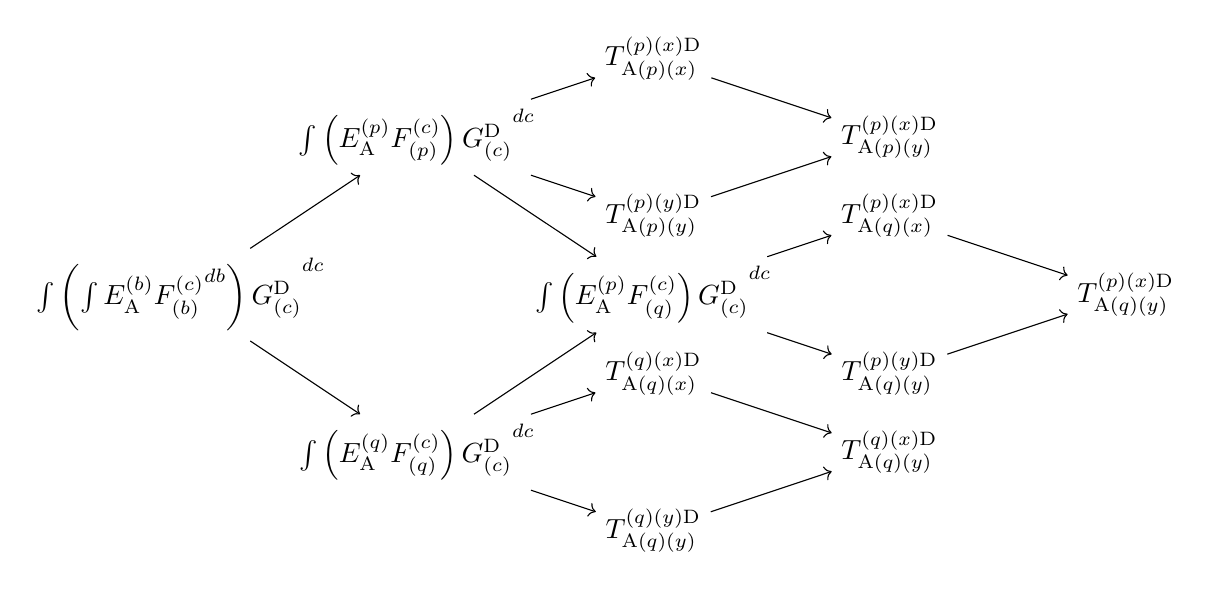
\begin{tikzpicture}
      \node (EFG1) at (0,4) {$\int {\left(\int {E_\AA^{(b)} F_{(b)}^{(c)}}^{db} \right) G_{(c)}^\DD}^{dc}$};

      \node (EFG2) at (3,6) {$\int {\left(E_\AA^{(p)} F_{(p)}^{(c)}\right) G_{(c)}^\DD}^{dc}$};
      \node (EFG3) at (3,2) {$\int {\left(E_\AA^{(q)} F_{(q)}^{(c)}\right) G_{(c)}^\DD}^{dc}$};

      \node (EFG4) at (6,4) {$\int {\left(E_\AA^{(p)} F_{(q)}^{(c)}\right) G_{(c)}^\DD}^{dc}$};
      \node (EFG5) at (6,1) {$T_{\AA(q)(y)}^{(q)(y)\DD}$};
      \node (EFG6) at (6,3) {$T_{\AA(q)(x)}^{(q)(x)\DD}$};
      \node (EFG7) at (6,5) {$T_{\AA(p)(y)}^{(p)(y)\DD}$};
      \node (EFG8) at (6,7) {$T_{\AA(p)(x)}^{(p)(x)\DD}$};

      \node (EFG9) at (9,2) {$T_{\AA(q)(y)}^{(q)(x)\DD}$};
      \node (EFG10) at (9,6) {$T_{\AA(p)(y)}^{(p)(x)\DD}$};
      \node (EFG11) at (9,3) {$T_{\AA(q)(y)}^{(p)(y)\DD}$};
      \node (EFG12) at (9,5) {$T_{\AA(q)(x)}^{(p)(x)\DD}$};

      \node (EFG13) at (12,4) {$T_{\AA(q)(y)}^{(p)(x)\DD}$};

      \draw[->] (node cs:name=EFG1) -- node[auto=left] {} (node cs:name=EFG2);
      \draw[->] (node cs:name=EFG1) -- node[auto=left] {} (node cs:name=EFG3);
      \draw[->] (node cs:name=EFG2) -- node[auto=left] {} (node cs:name=EFG4);
      \draw[->] (node cs:name=EFG3) -- node[auto=left] {} (node cs:name=EFG4);
      \draw[->] (node cs:name=EFG2) -- node[auto=left] {} (node cs:name=EFG8);
      \draw[->] (node cs:name=EFG2) -- node[auto=left] {} (node cs:name=EFG7);
      \draw[->] (node cs:name=EFG3) -- node[auto=left] {} (node cs:name=EFG6);
      \draw[->] (node cs:name=EFG3) -- node[auto=left] {} (node cs:name=EFG5);
      \draw[->] (node cs:name=EFG5) -- node[auto=left] {} (node cs:name=EFG9);
      \draw[->] (node cs:name=EFG6) -- node[auto=left] {} (node cs:name=EFG9);
      \draw[->] (node cs:name=EFG7) -- node[auto=left] {} (node cs:name=EFG10);
      \draw[->] (node cs:name=EFG8) -- node[auto=left] {} (node cs:name=EFG10);
      \draw[->] (node cs:name=EFG4) -- node[auto=left] {} (node cs:name=EFG11);
      \draw[->] (node cs:name=EFG4) -- node[auto=left] {} (node cs:name=EFG12);
      \draw[->] (node cs:name=EFG11) -- node[auto=left] {} (node cs:name=EFG13);
      \draw[->] (node cs:name=EFG12) -- node[auto=left] {} (node cs:name=EFG13);
    \end{tikzpicture}
    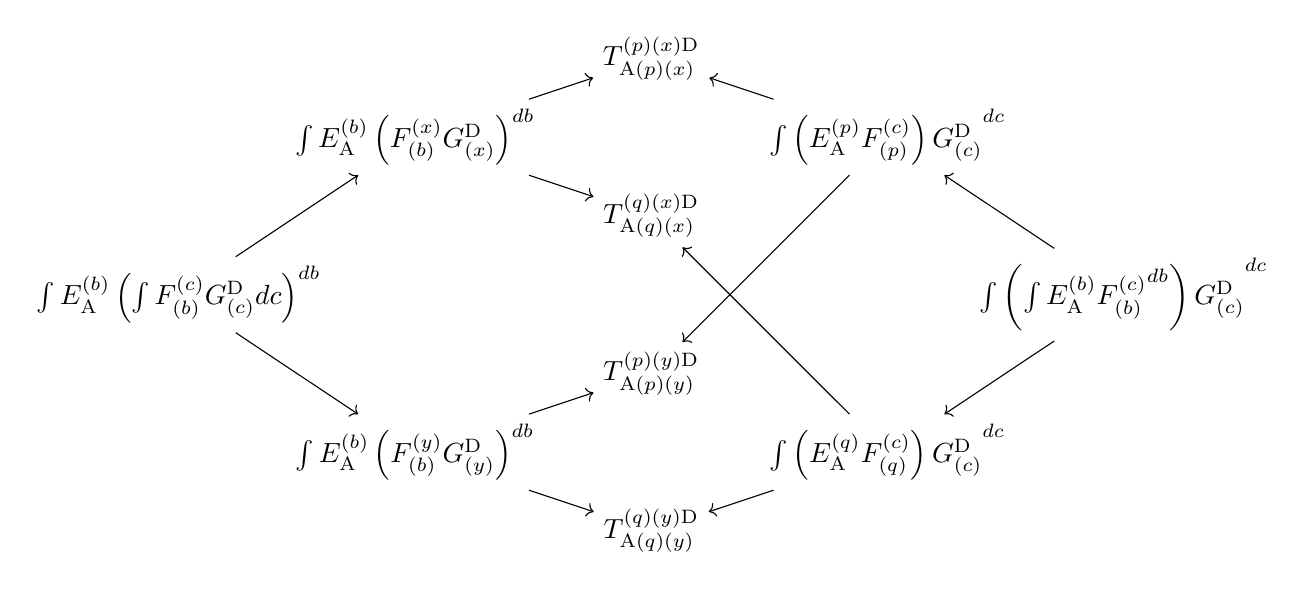
\begin{tikzpicture}
      \node (EFG1') at (12,4) {$\int {\left(\int {E_\AA^{(b)} F_{(b)}^{(c)}}^{db} \right) G_{(c)}^\DD}^{dc}$};

      \node (EFG2') at (9,6) {$\int {\left(E_\AA^{(p)} F_{(p)}^{(c)}\right) G_{(c)}^\DD}^{dc}$};
      \node (EFG3') at (9,2) {$\int {\left(E_\AA^{(q)} F_{(q)}^{(c)}\right) G_{(c)}^\DD}^{dc}$};

      \node (EFG1) at (0,4) {$\int E_\AA^{(b)} \left(\int F_{(b)}^{(c)} G_{(c)}^\DD dc\right)^{db}$};

      \node (EFG2) at (3,6) {$\int E_\AA^{(b)} \left(F_{(b)}^{(x)} G_{(x)}^\DD\right)^{db}$};
      \node (EFG3) at (3,2) {$\int E_\AA^{(b)} \left(F_{(b)}^{(y)} G_{(y)}^\DD\right)^{db}$};

      \node (EFG5) at (6,1) {$T_{\AA(q)(y)}^{(q)(y)\DD}$};
      \node (EFG6) at (6,3) {$T_{\AA(p)(y)}^{(p)(y)\DD}$};
      \node (EFG7) at (6,5) {$T_{\AA(q)(x)}^{(q)(x)\DD}$};
      \node (EFG8) at (6,7) {$T_{\AA(p)(x)}^{(p)(x)\DD}$};

      \draw[->] (node cs:name=EFG1) -- node[auto=left] {} (node cs:name=EFG2);
      \draw[->] (node cs:name=EFG1) -- node[auto=left] {} (node cs:name=EFG3);
      \draw[->] (node cs:name=EFG2) -- node[auto=left] {} (node cs:name=EFG8);
      \draw[->] (node cs:name=EFG2) -- node[auto=left] {} (node cs:name=EFG7);
      \draw[->] (node cs:name=EFG3) -- node[auto=left] {} (node cs:name=EFG6);
      \draw[->] (node cs:name=EFG3) -- node[auto=left] {} (node cs:name=EFG5);

      \draw[->] (node cs:name=EFG1') -- node[auto=left] {} (node cs:name=EFG2');
      \draw[->] (node cs:name=EFG1') -- node[auto=left] {} (node cs:name=EFG3');
      \draw[->] (node cs:name=EFG2') -- node[auto=left] {} (node cs:name=EFG8);
      \draw[->] (node cs:name=EFG2') -- node[auto=left] {} (node cs:name=EFG6);
      \draw[->] (node cs:name=EFG3') -- node[auto=left] {} (node cs:name=EFG7);
      \draw[->] (node cs:name=EFG3') -- node[auto=left] {} (node cs:name=EFG5);
    \end{tikzpicture}
  \end{center}
  ここで,エンドの普遍性により一意的な射$!$が存在する.
  \begin{center}
    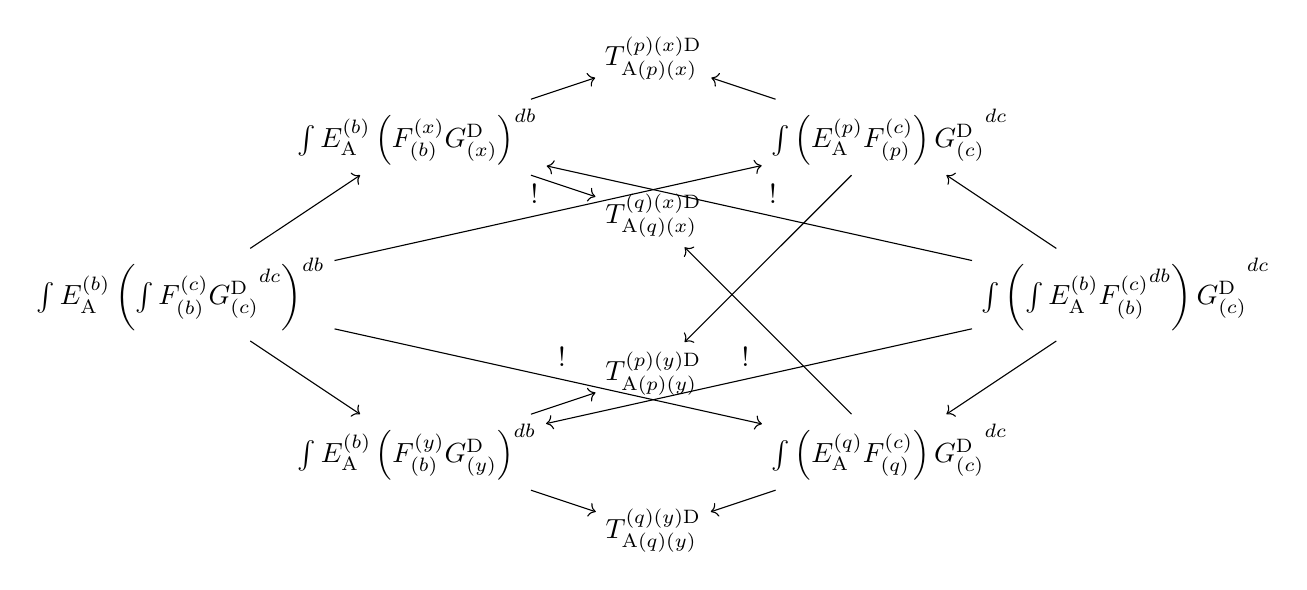
\begin{tikzpicture}
      \node (EFG1') at (12,4) {$\int {\left(\int {E_\AA^{(b)} F_{(b)}^{(c)}}^{db} \right) G_{(c)}^\DD}^{dc}$};

      \node (EFG2') at (9,6) {$\int {\left(E_\AA^{(p)} F_{(p)}^{(c)}\right) G_{(c)}^\DD}^{dc}$};
      \node (EFG3') at (9,2) {$\int {\left(E_\AA^{(q)} F_{(q)}^{(c)}\right) G_{(c)}^\DD}^{dc}$};

      \node (EFG1) at (0,4) {$\int E_\AA^{(b)} \left(\int {F_{(b)}^{(c)} G_{(c)}^\DD}^{dc}\right)^{db}$};

      \node (EFG2) at (3,6) {$\int E_\AA^{(b)} \left(F_{(b)}^{(x)} G_{(x)}^\DD\right)^{db}$};
      \node (EFG3) at (3,2) {$\int E_\AA^{(b)} \left(F_{(b)}^{(y)} G_{(y)}^\DD\right)^{db}$};

      \node (EFG5) at (6,1) {$T_{\AA(q)(y)}^{(q)(y)\DD}$};
      \node (EFG6) at (6,3) {$T_{\AA(p)(y)}^{(p)(y)\DD}$};
      \node (EFG7) at (6,5) {$T_{\AA(q)(x)}^{(q)(x)\DD}$};
      \node (EFG8) at (6,7) {$T_{\AA(p)(x)}^{(p)(x)\DD}$};

      \draw[->] (node cs:name=EFG1) -- node[auto=left] {} (node cs:name=EFG2);
      \draw[->] (node cs:name=EFG1) -- node[auto=left] {} (node cs:name=EFG3);
      \draw[->] (node cs:name=EFG2) -- node[auto=left] {} (node cs:name=EFG8);
      \draw[->] (node cs:name=EFG2) -- node[auto=left] {} (node cs:name=EFG7);
      \draw[->] (node cs:name=EFG3) -- node[auto=left] {} (node cs:name=EFG6);
      \draw[->] (node cs:name=EFG3) -- node[auto=left] {} (node cs:name=EFG5);

      \draw[->] (node cs:name=EFG1') -- node[auto=left] {} (node cs:name=EFG2');
      \draw[->] (node cs:name=EFG1') -- node[auto=left] {} (node cs:name=EFG3');
      \draw[->] (node cs:name=EFG2') -- node[auto=left] {} (node cs:name=EFG8);
      \draw[->] (node cs:name=EFG2') -- node[auto=left] {} (node cs:name=EFG6);
      \draw[->] (node cs:name=EFG3') -- node[auto=left] {} (node cs:name=EFG7);
      \draw[->] (node cs:name=EFG3') -- node[auto=left] {} (node cs:name=EFG5);

      \draw[->] (node cs:name=EFG1') -- node[auto=right] {$!$} (node cs:name=EFG3);
      \draw[->] (node cs:name=EFG1') -- node[auto=right] {$!$} (node cs:name=EFG2);

      \draw[->] (node cs:name=EFG1) -- node[auto=left] {$!$} (node cs:name=EFG3');
      \draw[->] (node cs:name=EFG1) -- node[auto=left] {$!$} (node cs:name=EFG2');
    \end{tikzpicture}
  \end{center}
  更にもう一度,エンドの普遍性を用いることで,
  \begin{center}
    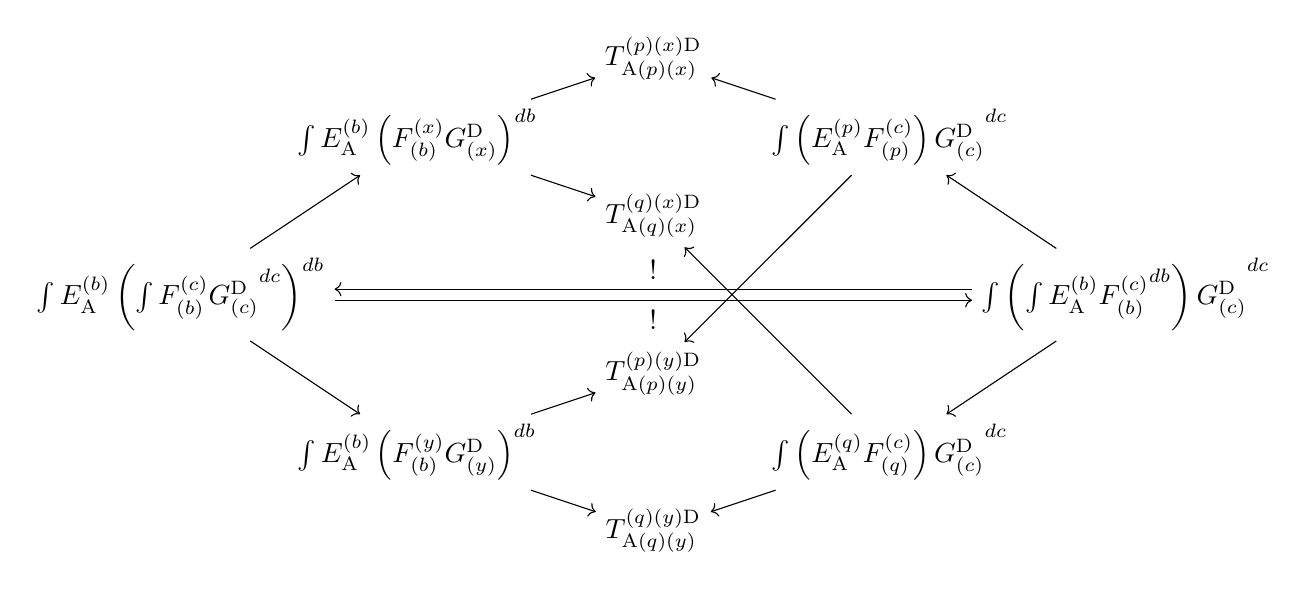
\begin{tikzpicture}
      \node (EFG1') at (12,4) {$\int {\left(\int {E_\AA^{(b)} F_{(b)}^{(c)}}^{db} \right) G_{(c)}^\DD}^{dc}$};

      \node (EFG2') at (9,6) {$\int {\left(E_\AA^{(p)} F_{(p)}^{(c)}\right) G_{(c)}^\DD}^{dc}$};
      \node (EFG3') at (9,2) {$\int {\left(E_\AA^{(q)} F_{(q)}^{(c)}\right) G_{(c)}^\DD}^{dc}$};

      \node (EFG1) at (0,4) {$\int E_\AA^{(b)} \left(\int {F_{(b)}^{(c)} G_{(c)}^\DD}^{dc}\right)^{db}$};

      \node (EFG2) at (3,6) {$\int E_\AA^{(b)} \left(F_{(b)}^{(x)} G_{(x)}^\DD\right)^{db}$};
      \node (EFG3) at (3,2) {$\int E_\AA^{(b)} \left(F_{(b)}^{(y)} G_{(y)}^\DD\right)^{db}$};

      \node (EFG5) at (6,1) {$T_{\AA(q)(y)}^{(q)(y)\DD}$};
      \node (EFG6) at (6,3) {$T_{\AA(p)(y)}^{(p)(y)\DD}$};
      \node (EFG7) at (6,5) {$T_{\AA(q)(x)}^{(q)(x)\DD}$};
      \node (EFG8) at (6,7) {$T_{\AA(p)(x)}^{(p)(x)\DD}$};

      \draw[->] (node cs:name=EFG1) -- node[auto=left] {} (node cs:name=EFG2);
      \draw[->] (node cs:name=EFG1) -- node[auto=left] {} (node cs:name=EFG3);
      \draw[->] (node cs:name=EFG2) -- node[auto=left] {} (node cs:name=EFG8);
      \draw[->] (node cs:name=EFG2) -- node[auto=left] {} (node cs:name=EFG7);
      \draw[->] (node cs:name=EFG3) -- node[auto=left] {} (node cs:name=EFG6);
      \draw[->] (node cs:name=EFG3) -- node[auto=left] {} (node cs:name=EFG5);

      \draw[->] (node cs:name=EFG1') -- node[auto=left] {} (node cs:name=EFG2');
      \draw[->] (node cs:name=EFG1') -- node[auto=left] {} (node cs:name=EFG3');
      \draw[->] (node cs:name=EFG2') -- node[auto=left] {} (node cs:name=EFG8);
      \draw[->] (node cs:name=EFG2') -- node[auto=left] {} (node cs:name=EFG6);
      \draw[->] (node cs:name=EFG3') -- node[auto=left] {} (node cs:name=EFG7);
      \draw[->] (node cs:name=EFG3') -- node[auto=left] {} (node cs:name=EFG5);

      \draw[->,transform canvas={yshift=2pt}] (node cs:name=EFG1') -- node[auto=right] {$!$} (node cs:name=EFG1);
      \draw[->,transform canvas={yshift=-2pt}] (node cs:name=EFG1) -- node[auto=right] {$!$} (node cs:name=EFG1');
    \end{tikzpicture}
  \end{center}
  よって
  $\displaystyle\int E_\AA^{(b)} \left(\int {F_{(b)}^{(c)} G_{(c)}^\DD}^{dc}\right)^{db} = \int {\left(\int {E_\AA^{(b)} F_{(b)}^{(c)}}^{db} \right) G_{(c)}^\DD}^{dc}$
  が示される.
\end{proof}
\begin{theorem}
  \begin{align*}
    \Delta_{(a)}^\CC F_\CC &= \int {\Delta_{(a)}^{(c)} F_{(c)}}^{dc}
  \end{align*}
\end{theorem}

\end{document}